\documentclass[oneside,14pt]{extarticle}
\usepackage[utf8]{inputenc}
\usepackage[T1,T2A]{fontenc}
\usepackage[english,ukrainian]{babel}
\usepackage{tempora}

\usepackage{amssymb,amsfonts,amsmath,amsthm,mathtext,textcomp}

\usepackage[includehead, headsep=0pt, footskip=0pt, top=2cm, bottom=2cm, left=2.5cm, right=1cm]{geometry}
\usepackage{indentfirst}
\usepackage[onehalfspacing]{setspace}
\usepackage[headings]{fancyhdr}
\usepackage{etoolbox}
\usepackage{flafter}
\usepackage{listings}

\usepackage{graphicx}
\usepackage{float}
\usepackage[center]{titlesec}
\PassOptionsToPackage{hyphens}{url}\usepackage{hyperref}
\usepackage{array}
\fancyhf{}
\renewcommand{\headrulewidth}{0pt}
\fancyhead[R]{\thepage}
\pagestyle{fancy}
\fancypagestyle{plain}{%
	\fancyhf{}
	\fancyhead{}
	\fancyfoot{}
	\fancyhead[RO]{\thepage}
	\fancyhead[LE]{\thepage}
	\renewcommand{\headrulewidth}{0pt}
	\renewcommand{\footrulewidth}{0pt}
}
\lstset{breaklines=true,showstringspaces=false}
\graphicspath{ {./pictures} }
\counterwithin{figure}{section}
\titlelabel{\thetitle.\quad}
\usepackage{tocloft}
\setlength{\cftsecnumwidth}{5em}
\setlength\parindent{1.25cm}
\usepackage{enumitem}

\begin{document}

\setcounter{page}{2}
\tableofcontents
\newpage

\section{Короткий опис бази практики}
Swisspan — провідний виробник дерев'яних плитних матеріалів, що використовує сучасні інформаційні технології для оптимізації виробничих процесів та управління якістю продукції. Штаб-квартира компанії розташована у Швейцарії, а виробничі потужності та офіси представлені в різних країнах світу.

Компанія заснована у 2005 році з метою забезпечення високоякісних дерев'яних плит для меблевої промисловості та будівництва. Swisspan відома своєю інноваційністю та екологічним підходом до виробництва, використовуючи передові технології та забезпечуючи відповідність найвищим стандартам якості.

\subsection{Фокусні галузі}
\begin{itemize}
	\item Меблева промисловість
	\item Будівництво
	\item Дизайн інтер'єру
	\item Експорт дерев'яних плитних матеріалів
\end{itemize}

\subsection{Технічні й програмні засоби}

Swisspan активно застосовує сучасні системи управління виробництвом (MES) та ERP-системи для автоматизації бізнес-процесів і підвищення ефективності роботи. Для контролю якості використовуються системи моніторингу, що забезпечують точність і надійність вимірювань на всіх етапах виробництва.

\subsection{Характер робіт, пов’язаних із застосуванням ІТ}

Робота в компанії включає розробку, впровадження та підтримку ІТ-рішень для автоматизації виробничих і бізнес-процесів, оптимізацію логістики, управління запасами та забезпечення високої якості продукції. Спеціалісти працюють над інтеграцією новітніх технологій, таких як Інтернет речей (IoT), для покращення виробничих процесів та зменшення витрат.

\subsection{Організація роботи в колективі}

Компанія підтримує відкриту та інклюзивну корпоративну культуру, заохочуючи співробітників до інновацій і професійного розвитку. Swisspan сприяє командній роботі та співпраці між різними відділами, забезпечуючи комфортні умови праці та можливості для навчання і підвищення кваліфікації.

\section{Постановка завдання роботи}
\begin{enumerate}
	\item Ознайомлення з базою практики.
	\item Ознайомлення з вимогами поставленого завдання.
	\item Аналіз процесів виробництва на деревообробному підприємстві.
	\item Визначення вимог до програмного забезпечення.
	\item Ознайомлення з мовою програмування Python та IDE PyCharm.
	\item Вивчення технології розробки штучного інтелекту з елементами машинного зору.
	\item Розробка програмного забезпечення для виявлення дефектів деревини за допомогою технологій штучного інтелекту та машинного зору.
	\item Тестування програмного забезпечення.
\end{enumerate}

\section{Опис проведених робіт}

\subsection{Опис програмних технологій і термінів}

\paragraph{Технологія NumPy}

NumPy — це бібліотека Python, що використовується для обчислень з масивами та матрицями, а також надає велику кількість математичних функцій для роботи з цими масивами. Вона є основою для наукових обчислень у Python і забезпечує високопродуктивні багатовимірні структури даних.

\begin{list}{-}{Основні можливості NumPy:}
	\item ndarray, Потужний об'єкт для роботи з багатовимірними масивами.
	\item Широкий набір функцій для виконання операцій на масивах.
	\item Інструменти для інтеграції з C/C++ та Fortran.
	\item Лінійна алгебра, фур'є-перетворення, випадкові числа. Вбудовані функції для виконання складних математичних обчислень.
\end{list}

\paragraph{Технологія SciPy}

SciPy — це бібліотека Python, що побудована на основі NumPy і надає додаткові можливості для наукових та технічних обчислень. Вона містить модулі для оптимізації, інтеграції, інтерполяції, спеціальних функцій, обробки сигналів та інших.

\begin{list}{-}{Основні можливості SciPy:}
	\item Функції для мінімізації та розв'язання нелінійних рівнянь.
	\item Інструменти для чисельного інтегрування.
	\item Функції для роботи з інтерполяцією даних.
	\item Функції для фільтрації та аналізу сигналів.
	\item Великий набір спеціальних математичних функцій.
\end{list}

\paragraph{Технологія Scikit-learn}

Scikit-learn (також відома як sklearn) — це бібліотека машинного навчання для мови програмування Python, яка надає інструменти для створення та тренування різноманітних алгоритмів класифікації, регресії та кластеризації. Вона є однією з найбільш популярних бібліотек для машинного навчання.

\begin{list}{-}{Основні можливості Scikit-learn:}
	\item Інструменти для різних видів класифікації, таких як логістична регресія та підтримувані вектори.
	\item Моделі для прогнозування, такі як лінійна регресія та градієнтний бустинг.
	\item Алгоритми для групування даних, такі як K-means та ієрархічна кластеризація.
	\item Методи для зменшення кількості ознак у наборі даних.
	\item Інструменти для оцінки ефективності моделей.
\end{list}

\paragraph{Технологія OpenCV}

OpenCV (Open Source Computer Vision Library) — це бібліотека з відкритим вихідним кодом для комп'ютерного зору та машинного навчання. Вона містить понад 2500 оптимізованих алгоритмів для обробки зображень і відео.

\begin{list}{-}{Основні можливості OpenCV:}
	\item Функції для роботи з різними операціями над зображеннями, такими як зміна розміру, фільтрація та обробка кольорів.
	\item Інструменти для захоплення, запису та обробки відеопотоків.
	\item Алгоритми для виявлення та розпізнавання облич, руху та інших об'єктів.
	\item Функції для калібрування камер та виправлення спотворень.
	\item Інструменти для побудови та тренування моделей машинного навчання.
\end{list}

\paragraph{Технологія Pillow}

Pillow — це бібліотека Python для роботи з зображеннями, яка є форком бібліотеки Python Imaging Library (PIL). Вона надає інструменти для відкриття, маніпулювання та збереження зображень у різних форматах.

\begin{list}{-}{Основні можливості Pillow:}
	\item Підтримка багатьох форматів зображень, таких як JPEG, PNG, BMP та інші.
	\item Функції для змінення розміру, обрізання, повороту та інших операцій.
	\item Інструменти для застосування різних фільтрів, таких як розмиття та підвищення різкості.
	\item Функції для роботи з палітрами кольорів та конвертації між різними кольоровими просторами.
	\item Інструменти для додавання тексту до зображень.
\end{list}

\subsection{Проектування архітектури та інфраструктури застосунку}

\begin{figure}[H]
	\centering
	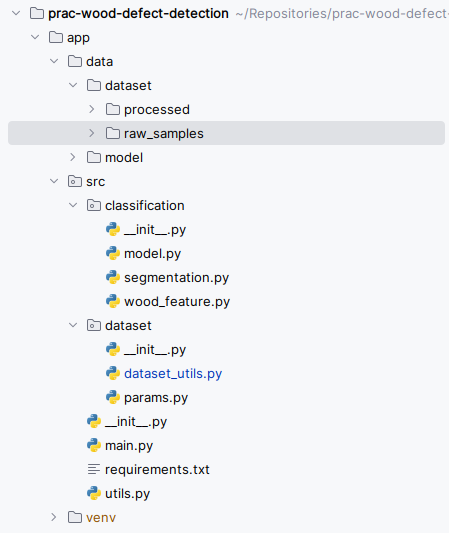
\includegraphics[scale=0.9]{1}
	\caption{Загальна структура проекту}
\end{figure}

\section{Практичні результати}

\subsection{Робота програми}

\begin{figure}[H]
	\centering
	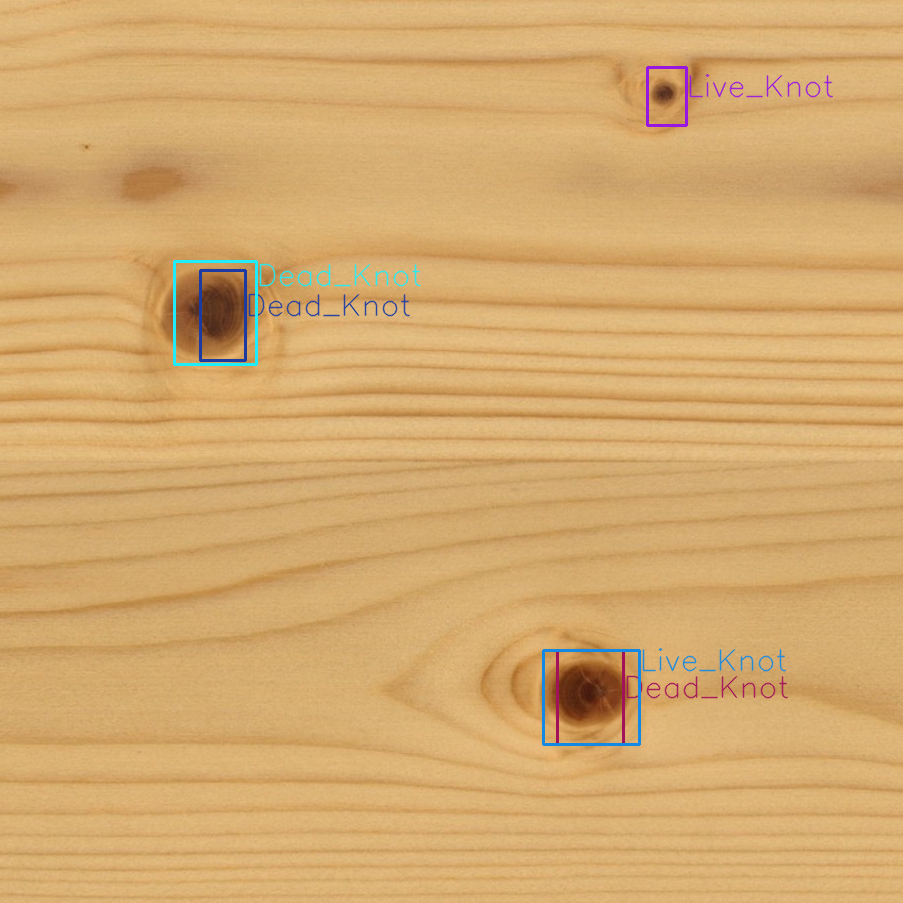
\includegraphics[scale=0.5]{2}
	\caption{Модифіковане зображення деревини з виділеними дефектами та їх класифікацією створене за допомогою програми}
\end{figure}

\subsection{Код програми}

\textbf{main.py}:
{\small\lstinputlisting{~/Repositories/prac-wood-defect-detection/app/src/main.py}}

\textbf{classification/model.py}:
{\small\lstinputlisting{~/Repositories/prac-wood-defect-detection/app/src/classification/model.py}}

\textbf{classification/segmentation.py}:
{\small\lstinputlisting{~/Repositories/prac-wood-defect-detection/app/src/classification/segmentation.py}}

\textbf{classification/wood\_feature.py}:
{\small\lstinputlisting{~/Repositories/prac-wood-defect-detection/app/src/classification/wood_feature.py}}

\textbf{dataset/dataset\_utils.py}:
{\small\lstinputlisting{~/Repositories/prac-wood-defect-detection/app/src/dataset/dataset_utils.py}}

\textbf{dataset/params.py}:
{\small\lstinputlisting{~/Repositories/prac-wood-defect-detection/app/src/dataset/params.py}}

\section*{Висновки про отримані результати}
\addcontentsline{toc}{section}{Висновки про отримані результати}

\section*{Список використаних джерел}
\addcontentsline{toc}{section}{Список використаних джерел}

\end{document}
